\section{Common Pipeline Results}

All results from the common pipeline were tested on the validation sets to avoid using the test set early.

\subsection{Multi-class Classification}

On the mini-MIAS dataset (multi-class classification problem), an accuracy of 50\% was achieved, with a confusion matrix (see Figure~\ref{fig:evaluation-common-CM-norm_basic-model_mini-MIAS-dataset}) indicating that the CNN is confusing cancerous cases together (benign and malignant), but can tell normal cases apart.

\begin{figure}[ht]
\centerline{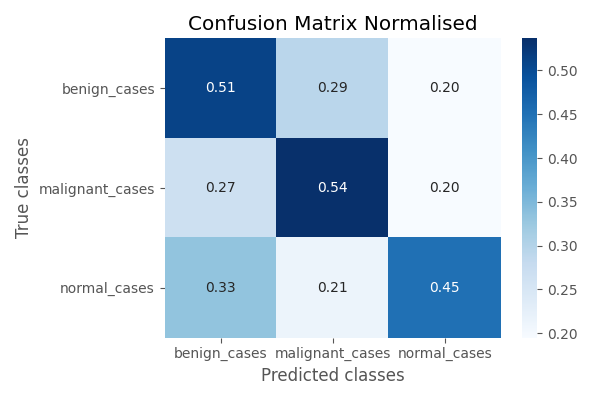
\includegraphics[width=0.8\textwidth]{figures/evaluation/common/CM-norm_basic-model_mini-MIAS-dataset.png}}
\caption{\label{fig:evaluation-common-CM-norm_basic-model_mini-MIAS-dataset}Normalised confusion matrix of the classification results after training on the mini-MIAS dataset.}
\end{figure}

\subsection{Binary Classification}

On the CBIS-DDSM dataset (binary classification problem), an accuracy of 65.36\% was initially achieved. Separating the types of mammograms between calcifications and masses revealed that higher accuracies could be achieved. Indeed, an accuracy of 70.36\% was reached when using only mammograms with masses, and 68.2\%  using only mammograms with calcifications (see Figure~\ref{fig:evaluation-cbisddsm-common-mass-vs-calc}).

\begin{figure}[h]
\centering
\begin{subfigure}{.5\textwidth}
  \centering
  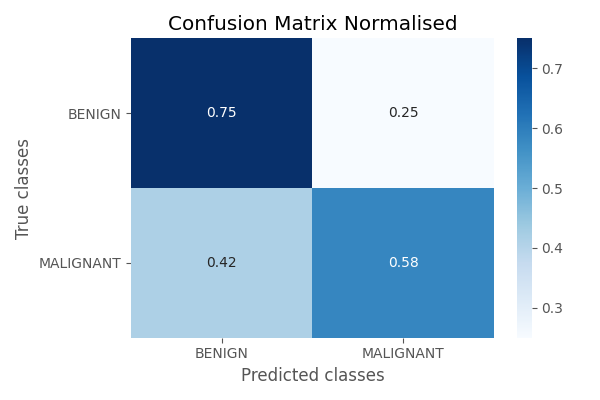
\includegraphics[width=\textwidth]{figures/evaluation/common/CM-norm_basic-model_CBIS-DDSM-dataset-Calc.png}
  \caption{Mammograms with calcifications (70.36\%).}
  \label{fig:evaluation-cbisddsm-common-calc}
\end{subfigure}%
\begin{subfigure}{.5\textwidth}
  \centering
  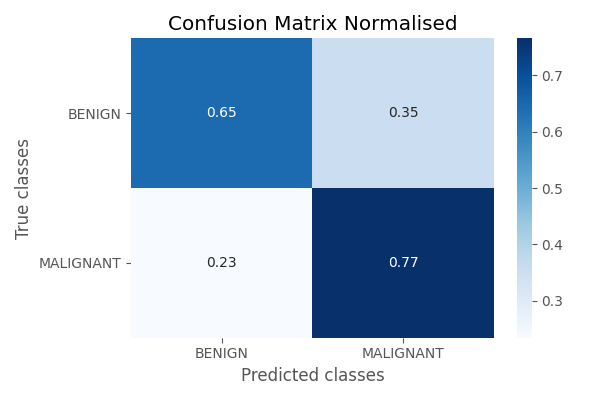
\includegraphics[width=\textwidth]{figures/evaluation/common/CM-norm_basic-model_CBIS-DDSM-dataset-Mass.png}
  \caption{Mammograms with masses (68.2\%).}
  \label{fig:evaluation-cbisddsm-common-mass}
\end{subfigure}
\caption{\label{fig:evaluation-cbisddsm-common-mass-vs-calc}Normalised confusion matrices between mammograms with calcifications and masses on the CBIS-DDSM dataset.}
\end{figure}

Minor optimisation attempts such as adding additional convolutional layers between the pre-trained VGG19 model and the fully connected layers lowered the accuracy to 55.07\%. Adding more convolutional and spooling layers before the VGG19 pre-trained model slightly increased the accuracy from 65.03\% to 65.36\%, but was much slower to train due to the increased number of trainable parameters that originated from the additional layers.

%%%%%%%%%%%%%%%%%%%%%%%%%%%%%%%%%%%%%%%%%%%%%

\section{Individual Optimisation Results}

Using more advanced models than VGG19, which is a sequential CNN, such as InceptionV3, yielded poor results and required much longer training times. Indeed, the evolution of the validation loss visualised in Figure~\ref{fig:evaluation-individual-inceptionv3-poor-training}  confirms that  the InceptionV3 model highly overfits the data, suggested an urgent need for regularisation techniques such as Dropout.\\

\begin{figure}[ht]
\centerline{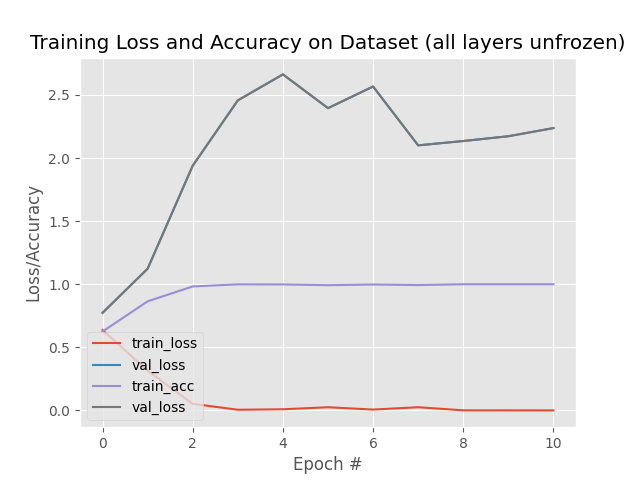
\includegraphics[width=0.8\textwidth]{figures/evaluation/individual/InceptionV3-poor-training.png}}
\caption{\label{fig:evaluation-individual-inceptionv3-poor-training}Evolution of validation loss during training of the InceptionV3 model on the CBIS-DDSM dataset.}
\end{figure}

Potential future comparisons:
\begin{itemize}
    \item Different CNN models (VGG19, ResNet50V2, InceptionV3, Xception)
    \item Using transfer learning (pre-trained model on ImageNet)
    \item Using different types of mammograms (calcifications only, masses only, both)
\end{itemize}

\subsection{Dataset Transfer Learning}

Train model on small binarised mini-MIAS dataset, dropping all normal cases and retaining only benign and malignant cases).\\

Accuracy not improved, loss is immediately optimal, so perhaps does not  get chance to explore new positions from random weight initialisation.\\

Same speed as without transfer learning, just 1-2 epochs less for large errors, but it is the number of maximum  epochs and early stopping conditions that dictate the runtime.

\subsection{Different Types of Mammograms}

Using the CBIS-DDSM dataset, all, calc and mass

same learning rate, dropout layers 0.2